\section{Study Design}
\label{cha:studydesign}
As previously stated, benchmark suites require large cloud environments to run and analyze performance issues. For this purpose, this research uses an open-source time series database system called VictoriaMetrics to run both application benchmarks and microbenchmarks. The system was selected because it provides built-in microbenchmarks and application benchmarking capabilities. This research aims to determine to what extent the microbenchmarks can predict a change in the application benchmarks’ performance and whether using ridge regression to anticipate performance regressions or optimizations. Enabling developers to detect issues faster, save time, and decrease bad releases to production.  \\
This study follows a structured experimental approach, executing both benchmarking types under controlled and reproducible conditions in a cloud-based environment. It also examines whether a predictive model, specifically ridge regression, can effectively anticipate application performance trends with the microbenchmark results. \\
This research starts by running the application benchmark to obtain the mean query rate values that the ridge regression should be able to predict using the microbenchmark results. After this step, the complete microbenchmark will be run; then, we optimize the microbenchmark suite by performing a collinearity reduction so the ridge regression can use the resulting features. This optimization provides reliable data this research uses to predict the application benchmark performance. \\
This research follows three main phases to run the experiments: setup, installation, and running. It executes these three phases to configure the virtual machines with the right version of the \ac{SUT}. The first phase, setup, involves configuring the virtual machines (\ac{VM}s) required for the experiments. In this phase, we use Ansible to set up and manage all the virtual machine instances.  \\
\cref{fig:benchmarks-setup} shows both the application benchmark and microbenchmark setup. As shown in \cref{fig:applicationBenchmark-setup}, we create two instances for the application benchmark: one for the \ac{SUT} and one for the benchmarking client, whose primary responsibility is generating the load for the \ac{SUT}. Having two separate instances ensures that the \ac{SUT}’s performance is not affected by resource consumption related to workload generation. Furthermore, \cref{fig:microbenchmark-setup} shows that no client is created for the microbenchmark because we do not need to generate data. Making the microbenchmarks’ setup simpler where we only need to run the performance test in the \ac{SUT}.

\begin{figure}[!htbp]
    \captionsetup[subfigure]{list=true}
    \centering
    % -- Row 1: two subfigures --
    \begin{subfigure}[b]{0.49\textwidth}
        \centering
        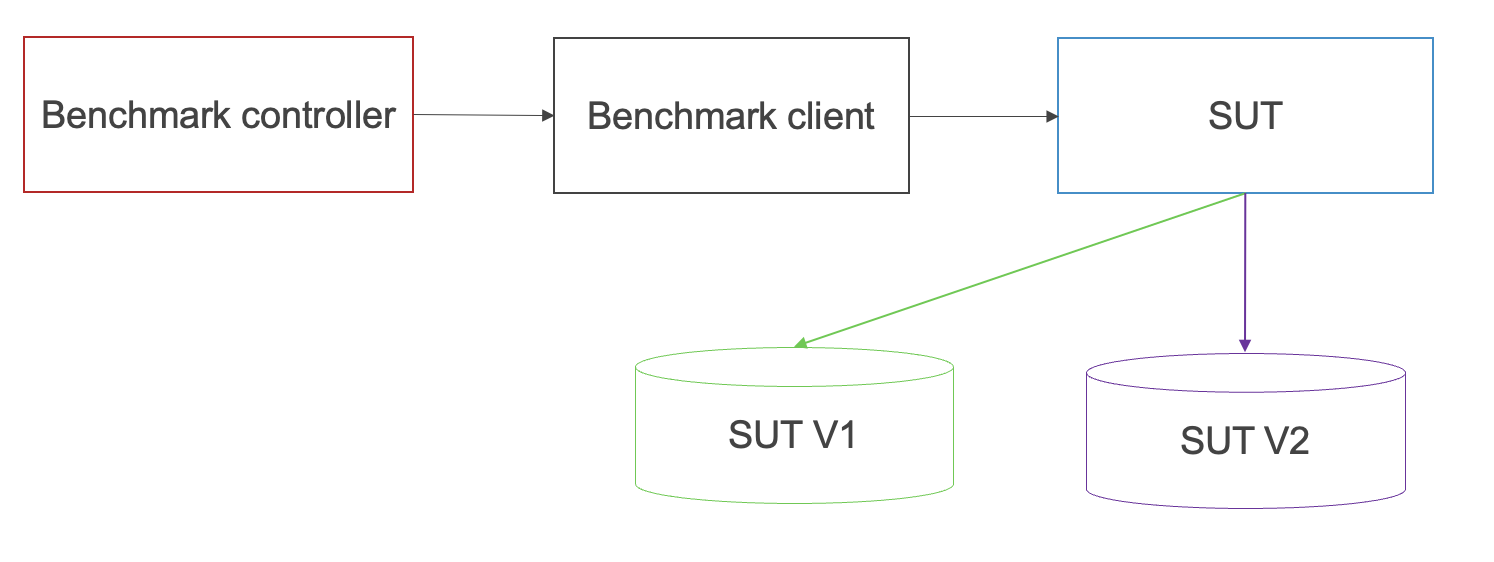
\includegraphics[width=\textwidth]{figures/Application setup.png}
        \caption{Application Benchmark Setup}
        \label{fig:applicationBenchmark-setup}
    \end{subfigure}
    \hfill
    \begin{subfigure}[b]{0.49\textwidth}
        \centering
        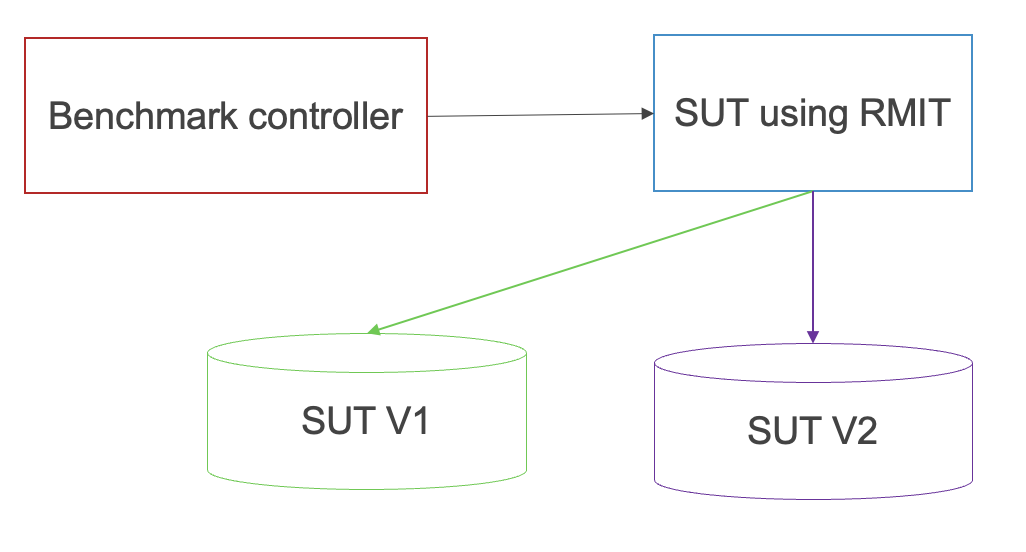
\includegraphics[width=\textwidth]{figures/Microbenchemark setup.png}
        \caption{Microbenchmark Setup}
        \label{fig:microbenchmark-setup}
    \end{subfigure}
    \caption{Benchmarks setup}
    \label{fig:benchmarks-setup}
\end{figure}

Additionally, we create another instance called a controller in both setups. The controller instance orchestrates the experiments with a startup script that will parallel start the application benchmark and the microbenchmarks. Since the experiments are done in parallel, the controller will start the application benchmark and the microbenchmarks in different terminal processes. Having the controller is helpful to avoid having control over the experiments on the local computer; since the experiments take a long time to complete, one will likely close the computer, restart, or close the terminal without the experiments finishing, thus losing the data collected. Therefore, having this approach prevents local machine disruptions that could lead to data loss or invalid results if the experiments were run locally. \\
Once the setup is complete and we created all the instances, the second phase starts, the installation phase. In this phase, we install the required software into the instances on each virtual machine. Key installations include GO, Docker, Git, benchmarking tools like VictoriaMetrics and GoAPIBenchmarkingScore (\ac{GoAbs}), and a Time series benchmark suite (\ac{TSBS}). All the virtual machines in both the microbenchmark and application benchmark are set up to run Debian-11 as the operating system and are deployed to the zone euro-west1-b. After we install the required tooling, we run another Ansible command to configure the \ac{SUT} for both the application benchmark and the microbenchmark.  \\
Lastly, the third phase is running the experiments. This phase comes into place once the installation is done. In this stage, the controller instance will be restarted, and the startup script will be triggered to execute the application benchmark and the microbenchmarks using benchmarking techniques, such as duet benchmarking for application benchmarks and Randomised Multiple Interleaved Trials (\ac{RMIT}) for microbenchmarks, to reduce external noise and improve data reliability. \\
After running the benchmarks, we collect the data from the experiments and analyze the results, which will be used to train and validate a ridge regression model. 


\subsection{Application benchmarks}
For the application benchmark, this research uses an open-source tool called the Time Series benchmark suite, further referred to as \ac{TSBS}. This tool was created to measure the performance of different Time Series databases, giving the developer a chance to compare them; one of those is VictoriaMetrics, which makes it easier to deploy the experiments to test the research question. \ac{TSBS} comes with predefined useCases to generate the workload for the \ac{SUT}s; depending on the useCase selected, one can get different workload data; one of the available useCases in \ac{TSBS} for VictoriaMetrics is the useCase "DevOps", which aligns perfectly with this research, as the main objective of this research is to allow developers to detect performance regressions faster. \\
As previously stated, application benchmarks deploy a \ac{SUT} to a real environment to detect performance changes. Therefore, to mimic a realistic setup, we set virtual machines (\ac{VM}s) from scratch for the application benchmarks and created 2 \ac{VM}s. The first runs the \ac{SUT},  and the second is a client in charge of generating and inserting the artificial loads into the \ac{SUT}. The reason behind this is to prevent the resources of the \ac{SUT} from being affected by the generation of artificial loads and their insertion in the \ac{SUT}. Thus, by separating this into two \ac{VM}s, we can guarantee that the \ac{SUT} only has the application load that will be tested. For the application benchmarks’ configuration, we use Docker to pull the image for each version configured in the configuration file and run the two Docker containers. \cref{tab:vm_configurations} shows the resources used for the virtual machines' configuration. \\
\begin{table}[ht]
    \centering
    \begin{tabular}{lccc}
        \toprule
        \textbf{Resource} & \textbf{Controller} & \textbf{Client} & \textbf{System Under Test (SUT)} \\
        \midrule
        Machine Setup & e2-medium & e2-standard-8 & e2-standard-4 \\
        Virtual CPUs & 2 & 8 & 4 \\
        Memory (GB) & 4 & 32 & 16 \\
        Disk Size (GB) & 50 & 50 & 50 \\
        \bottomrule
    \end{tabular}
    \caption{Virtual machine configurations for application benchmark}
    \label{tab:vm_configurations}
\end{table}
We use the e2-standard-4 virtual machine configuration, which allows us to divide four virtual \ac{CPU}s and 16 GB of memory into two Docker containers. Docker helped us limit the allowed CPU resources for the application benchmark, resulting in each container having 1.5 virtual \ac{CPU}s and 6 GB of memory available. This setup guarantees that the system under test is maxed out with artificial workloads and provides reliable results, ensuring that the system is under stress to be able to see and analyze its limits and detect performance changes. At the same time, we also have to guarantee that the client is not using over \text{60\%} of the resources to ensure that the client is not a bottleneck in this experiment. we changed the default disk size to 50 GB. With this setup in the application benchmark, we take advantage of the Duet benchmarking technique. We run the two versions of Victoria metrics in the same virtual machine using Docker to limit the resources available to each container. Hence, they have the same \ac{CPU} and \ac{RAM} to reduce external noise in the data generated by the application benchmark, ensuring that both versions of the \ac{SUT} operate under identical conditions. \\
\begin{table}[ht]
    \centering
    \begin{tabular}{l r}
        \toprule
        \midrule
        Number of Simulated Servers & 800 \\
        Sending Interval & 60s \\
        Simulated Duration & 120h \\
        Batch Size & 75 \\
        Number of Group-By Queries & 8,640 \\
        Number of Workers & 10 \\
        \bottomrule
    \end{tabular}
    \caption{Application benchmark parameters}
    \label{tab:applicationBenchmarkParameters}
\end{table}
This research executes the application benchmark in two steps. First, the benchmarking client generates data, which stresses the \ac{SUT}. Then, running the \ac{TSBS} workload using the DevOps use case generates data, as shown in \cref{tab:applicationBenchmarkParameters}, generates the data over five days with an interval of 60 seconds and uses the same interval to generate the queries that will be executed against the \ac{SUT}. Once the benchmark client generates the data for the 8640 queries, the next step is to insert the data into the \ac{SUT}. We run two terminal processes to insert the data into each Victoria metrics version. Next, we will wait for the data to be inserted into the two versions and give the \ac{SUT} 60 seconds to stabilize. \\
After this, we again create two new processes that will run the Group-by queries against each version of Victoria metrics, which conclude the execution of the application benchmark. Each experiment is repeated 10 times on the same pair of versions, e.g., v1.104- v1.105, another 10 times for v1.105-v1.106, 10 times for v1.106-v1.107, 10 times for v1.107- v1.108, and 10 times for v1.108-v1.109. We process the output files for each version and export the results to calculate the average load latency and the average Group-by query execution latency. We sum those values, resulting in the application benchmark’s average latency, and then compare them in the following section with the microbenchmark’s results to train and validate a ridge regression model. 

\subsection{Microbenchmarks}
On the other hand, to run the microbenchmarks, we use the Go API Benchmarking Score, also known as \ac{GoAbs}. This tool lets us execute microbenchmarks multiple times, having multiple iterations in each microbenchmark. The microbenchmarks were also executed into two versions, similar to the application benchmarks, to have more reliable results. \ac{GoAbs} allows us to enter a configuration file where one can define which functions of the microbenchmarks will be executed and how many times each function needs to be run. Additionally, one can determine how often we want the complete microbenchmark suite executed. Determining the execution time helps us obtain more data, giving us more reliable results. Furthermore, Grambow et al. \cite{grambow} adapted ABS by making some changes in the code and allowing two projects to be compared; the code changes consisted of only considering the common microbenchmarks in both versions to avoid analyzing irrelevant microbenchmarks and reducing costs and waste of resources. \\
For the microbenchmark setup, we only need to ensure that we have correctly installed GO so that the tool \ac{GoAbs} can be run correctly. In this case, as shown in \cref{tab:vm_configurations_micro}, we used the e2-standard-2 Virtual machine configuration, which provides two virtual \ac{CPU}s and 8 GB of memory. \\
This research follows the methodology proposed by Grambow et al. \cite{grambow} to execute the microbenchmarks. We will run the benchmark suite 3 times and each microbenchmark 5 times per run, giving us 45 measurements per microbenchmark. Considering that as Grambow et al. \cite{grambow}, this research executes two versions, obtaining a result of 45 measurements per microbenchmark per version. \\
Similar to the application benchmark, the microbenchmarks for the two versions are executed on the same virtual machine. The process for the microbenchmarks is much simpler; we clone the two different versions defined in the configuration file and execute \ac{GoAbs}to start running them. Lastly, to obtain accurate results, we use \ac{RMIT} which allows us to compare two microbenchmark versions fairly to avoid bias and reduce the probability of having the same results
\cite{japke2023earlymicrobenchmarkcatches}. \\
\begin{table}[ht]
    \centering
    \begin{tabular}{lccc}
        \toprule
        \textbf{Resource} & \textbf{System Under Test (SUT)} \\
        \midrule
        Machine Setup & e2-standard-2 \\
        Virtual CPUs & 2\\
        Memory (GB) & 8  \\
        Disk Size (GB) & 50 \\
        \bottomrule
    \end{tabular}
    \caption{Virtual machine configurations for microbenchmarks}
    \label{tab:vm_configurations_micro}
\end{table}

\subsection{Model Selection}
Performance prediction models help developers anticipate how software changes will affect system performance. To predict the application benchmark performance based on the microbenchmarks, we employed a multivariate linear regression model, more precisely, the ridge regression model. This model was selected because one of its primary properties is that it penalizes feature collinearity by incorporating a regularization strategy to remove it \cite{mcdonald2009ridgeregression}.  \\
Vrigazova \cite{vrigazova2021proportion} suggests splitting data into training and test data by allocating \text{80\%} for training and \text{20\%} for testing data. Therefore, this research will follow this suggestion after performing the data pre-cleanup. Then, we will fit the data into the model and apply the ridge regression. Once we obtain the quality metrics of the model, R-squared, and \ac{MSE}, we plan to load data that the model had never seen to test how accurate the predictions will be. As the \ac{SUT} obtains more releases, the likelihood of the microbenchmarks features changing is considerably high; therefore, we needed to make sure that the features that we trained to model with were present within any newly provided data in order to be able to use the model to predict the application benchmark. If we do not find the needed features, we will add 0 as the corresponding value, allowing the model to ignore this feature without compromising its predictions. 